\chapter{Investigation of Visualization Tools using a Feature Classification Scheme}
\label{chap:Tools}

In this section we analyze selected visualization tools and their ability to visualize large time-oriented data. Therefore, the database metrics were compared for each tool. Database metrics are part of the definition of visual scalability and describe how tools scale to large data sets. A detailed discussion can be found at section \ref{databasemetrics}. Moreover, we developed a classification scheme which is based on the collected success criteria of chapter \ref{chap:BIV} and ranked the tools according to this classification scheme. \\*

\section{Selection of Tools}\label{tool:selection}
The tools were selected based on their relevance in business. Nowadays, businesses strive to do self-service data science\cite{Russom2011,Parenteau2016,visualization2012making,curran2005self}. Therefore, they use self-service tools which are characterized by a graphical user interface (GUI), low prior programming skills and the universal use. The GUI enables non computer scientists to analyze data by the help of the human visual system. Based on the Magic Quadrant for Business Intelligence and Analytics Platforms 2017 \cite{Sallam2017} Qlik, Tableau and Microsoft are the leading visionaries of BI Vendors. All of these tools are \textit{commercial} fee-based tools in the business context. Their strength lies in the user support and their universality. \cite{ITCentralStation} as a crowdsourcing recommendation platform for BI tools confirmed Gartner's assessment as Tableau, Qlik, Oracle, Microsoft Power BI and IBM Cognos ranked among the first five places. \\
Qlik, Tableau and Power BI are ranked as BI tools but at the same time they fulfill all criteria to call themselves visualization tools (\ref{tools}).
Thus, we chose the tools: Power BI, Tableau and Qlik Sense (QS).\\
Moreover, we added d3.js as it fulfills the criteria for visualization tools. d3.js is an open-source JavaScript library and offers a wide range of visualization possibilities. \\


%Nevertheless, market relevance reports from research and advisory companies such as Gartner, Forrester, Barc usually do not publish detailed scoring models.  Thus, the ranking might not be appropriate to our needs.


\iffalse
ADV in business context requires software that is able to scale visualization in an "effective manner"\cite{Russom2011}. Offering ADV techniques, parameterization, interaction and analytical methods such as data abstraction\cite{Tegarden1999,Aigner2011,Eick2002,Zhanga} are core functions of ADV software. \\*
\textbf{The Role of APIs}
Commercial software tends to need more time for the development and integration of advanced visualization for large data\cite{Zhanga, Simon2014}. To bridge the gap, vendors started to offer a bunch of APIs to expand the visualization functions. 
% data load for BigData: 
\textbf{Software not included in this work}
As the goal of this work is to compare visualization tools in business we only consider software which is 
\begin{enumerate}
    \item generic: not specialized to one domain
    \item integrates visualization features
\end{enumerate}

Furthermore, the software needs visualization features, the ability to present time-dependent data. Software with one of the following items is intentionally not considered: 
\begin{enumerate}
    \item Software that only presents one-dimensional data. 
    \item Software that is specialized to data mining.
\end{enumerate}
\fi

\textbf{Qlik Sense: }
Qlik Sense is the self-service product of Qliktech. Qliktech was founded in 1993 with the goal to "mimic how the brain works."\cite{qlikHistory}. They offer five products(QS, QS Cloud, QlikView, QlikView NPrinting, Qlik DataMarket) and the Qlik Analytics platform. QS 1.0 was released in September 2014 for visual analytics. 
Self-Service data visualization describes the approach to encourage a broad public to do data analysis with easy-to-use tools.\\
\textbf{Power BI: }
Microsoft Power BI came alive in September 2013. It is divided in the three services Power BI Mobile, Power BI Desktop and Power BI service. Power BI Mobile access reports by a portable device. Power BI Desktop is a business analytics suite for creating visualizations and reports and Power BI service publishes reports. We are concentrating on Power BI Desktop.\\
\textbf{Tableau: }
Tableau was founded in 2003 out of a university project. Tableau sells three main products: Tableau Desktop, Tableau Public and Tableau Server.\\ 
\textbf{d3.js: }
d3.js is a JavaScript library used for visualization. It visualizes data based on SVG, HTML5 and CSS and binds data to existing web elements in alignment with the Document Object Model (DOM).  Data Handling is managed by the underlying data source, data modeling can be handled by other JavaScript libraries such as node.js. A good overview how d3.js works is given in \cite{Meeks}. 
We chose d3.js as it is a data visualization tool with interaction. As it is free it becomes an alternative to commercial tools.\\


\section{Scalability of visualization tools}\label{tool:scalability}
Visual scalability of visualization tools is measured by the \text{visualization characteristics} and the \textit{database metrics}. Moreover, as discussed in \ref{chap:BIV} scalability is enhanced by analytical methods and interaction techniques.

\subsection{Database metrics}
Database metrics are defined as the size of the database which can be handled by tools\cite{Eick2002}. One possibility to measure the database size are the number of lines which can be loaded into the tool. Another approach to measure database metrics are the maximum number of rows which can be loaded into a visualization.
\par
While \textbf{d3.js}, \textbf{Power BI} and \textbf{Tableau} have no limitations how many data can be loaded, \textbf{QS} inherits the data load limitations of Qlik View: A QS document cannot have more than 2,147,483,648 distinct values in one field. This limitation still allows Qlik to handle large and huge data sets according to our definition. Moreover, 2 billion data points exceed the limit of screen pixels. But nevertheless, QS is outperformed by d3.js, Power BI and Tableau in this particular case.
\\*\\*
In context of visualization the number of rows which are loaded into a visualization is a determining factor for scalability. For large data the user expects to load all data he wants the tool to load. However, some tools limit the initial number of rows and the user has to write additional code. This effects the easy-of-use negatively.
QS limits the initial fetch to 10.000 but gives the opportunity to fetch more data if needed. \textbf{d3.js}, \textbf{Power BI} and \textbf{Tableau} currently have no limit for rows in visualization.
Again QS stays behind d3.js, Power BI and Tableau.

\subsection*{More than database metrics}
With the current development in technology, data management shifted from importing csv-files or Excel Spreadsheets to storing data sets in technologies such as clouds or databases.
Therefore, most of the visualization tools provide data engines, an underlying software component which manages the data. Thus, the tool performance depends at the following factors:
\begin{enumerate}
    \item Hardware Resources
    \item the underlying engine
    \item perceived performance 
\end{enumerate}
Out of the three factors visualization tools are in charge of the connection to the \textit{the underlying engine} and partially for the perceived performance. As perceived performance is also influenced by psychology and thus, independent of visualization tools, we are focusing on the underlying engine.
In our understanding of visual scalability Eicks definition of database metrics needs to be adjusted in a way that it meets the characteristics of tools today. Thus, we expand \textbf{database metrics} by the ability to integrate to the underlying engine.

\textbf{The underlying Engine: In-memory versus Real Time Connection}
In-memory techniques store their data inside the RAM while real time technologies work directly on the database.
With large data sets in-memory technologies might not be feasible. Even though working in-memory is faster than working directly at the database. With a smaller subset of large databases working in-memory might be the better option. 
\textbf{QS} data engine (QIX Engine) and \textbf{Power BI} use in-memory columnbased technology. While the data engine processes calculation the RAM may be temporarily allocated. Thus, QS is limited by the primary memory of the computer. \textbf{Power BI} also connects live to clouds and on premises similar to \textbf{Tableau} offers in-memory technology as well as live connection. With live connection the data analysis queries the database directly. Data extracts can be created to work in-memory. The limits for data extracts are not published but Tableau Public, the free version of Tableau, recently extended the limit of 1 mio. rows to 10 mio. rows in-memory. 
For working with large data sets Tableau again outperformed QS and Power BI.\\*
\textbf{Connection to multiple data sources}
With large data sets data is distributed about several places. The ability to connect to multiple databases impacts the scalability. All of the tools can connect to multiple data sources. In future work, a performance review for the connection of the tools to multiple data sources is recommended.\\*
\textbf{Incremental Loading}
With large data sets tools might be overstrained with loading the whole data sets at once. Strategies to tackle this problem are incremental load. \textbf{QS} uses a custom data model called .QVD files. In .QVD files data is highly compressed and allows incremental loading. Tableau allows the incremental refresh of data extracts which adds only new rows to the extract. Power BI does not offer the option of incremental loading. 
\textbf{Further Aspects}
Scalability of tools can also be measured in terms of users and delivery which goes beyond our scope.




\subsection{Visualization Characteristics}

\textbf{The classification scheme}\label{tool:classification}\\*
The tools basis of assessment concerning \textit{visualization characteristics} is a classification scheme. In chapter \ref{BIV} the importance of \textit{data reduction (Analytical Techniques), advanced visualization techniques (Visualization Techniques) and interaction techniques (Interaction Techniques)} has been shown. These three aspects are assessed according to two business relevant criteria for self-service tools: the criterion of completeness and the criterion of required programming skills. The factor \textit{completeness} serves as indicator how many features can the business user achieve with this tool. Completeness in aggregation metaphors displays how many visualization techniques include aggregation metaphors. Yet, completeness is difficult to measure. Thus, we compare completeness by relative comparison.\\*
\begin{table}[H]
	\caption[Tool Completeness]{Criteria Completeness: extend to which assessed aspect is implemented in tool}
	\label{programming-skills}
	\begin{tabu}{cl}
	\toprule
	Points & Criteria\\
	\midrule
	0 & Not existing\\
	1 & partially implemented \\
	2 & fully implemented \\
	\bottomrule
	\end{tabu}
\end{table}

The consideration of programming skills in business is important as the standard business user of the visualization tool may have few programming knowledge (compare \ref{tasks}). Moreover, programming skills are connected with investment costs. The higher the required programming skills the higher are the investment costs. On a scale programming skills are measured by the required user knowledge to achieve a feature. Least effort is needed when the tool offers the feature automatically. The next step is to embed a feature via drag and drop. This step still does not require any programming skill. On the next level programming knowledge is required but in a popular programming language. A popular programming language such as R, Java, JavaScript, python, C can used in other environments as well which increases the probability that the user knows the language. The most complex level is when a feature can only be implemented by a tool-specific programming language. Here, we assume that a tool-specific language requires additional training effort. 
\begin{table}[H]
	\centering
	\caption[Programming-Skills for Tools ]{Criteria Required Programming-Skills to use the assessed aspect}
	\label{programming-skills}
	\begin{tabu}{cl}
	\toprule
	Points & Criteria\\
	\midrule
	1 & Feature can be programmed, but in a tool-specific programming language\\
	2 & Feature can be programmed in a popular programming language (R,JavaScript,Java)\\
	3 & Available by drag and drop \\
	4 & Automatic support by tool\\
	\bottomrule
	\end{tabu}
\end{table}

The criteria completeness and programming skills have been combined in the tool criteria score (TCS). Each feature of the tool has been assigned a tuple consisting of (Programming Skills, Completeness). If the assessed aspect did not exist 0 was assigned.
Based on the assessment of different features  we draw our conclusion (\ref{conclusion}).

\todo{Achse anpassen}
%example grid
\begin{figure}[H]
\centering
\scalebox{.75}{
    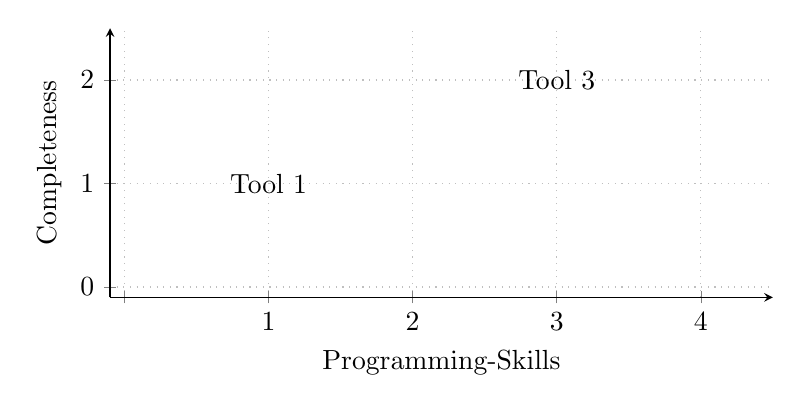
\begin{tikzpicture} 
        \begin{axis}[
        enlarge x limits=false,
        enlarge y limits=false,
        axis y line     = left,
        axis x line     = bottom,
        grid,
        grid style = {color=gray!50, dotted},
        width = 10cm, 
        height = 5cm,
        xticklabels={,,1,2,3,4},
        yticklabels={,0,1,2},
        xmin       = -0.1, domain = 0:4, xmax = 4.5,
        ymin       = -0.1, domain = 0:2, ymax = 2.5,
        xlabel={Programming-Skills},
        ylabel={Completeness}
        ]

        \node at (axis cs: 1,1)   {Tool 1};
        \node at (axis cs: 3,2)   {Tool 3};
        \end{axis}
    \end{tikzpicture}}
    \caption{Tool Criteria Score (TCS)} \label{classification}
\end{figure}





\iffalse
\subsection*{R}
\textbf{Analytical Techniques}\\
Out of the five tools R has the most extensive offer of analytical methods for time-series data. It is possible to detect patterns such as outliers with tsoutliers\cite{Chen1993} and clusters with tsclust\cite{Manso2015}, do advanced analytics with tswge\cite{tswge} and forecasting with zra\cite{zra}.
\textbf{Visualization Techniques}\\
R supports standard visualization such as histograms, line charts and scatter plots. Advanced visualization techniques for large data sets 
\textbf{Aggregation}\\*
In the maps-package R offers the possibility to adjust the resolution with the parameter resolution. Resolution 0 maps the whole database whereas a higher resolution collapes data points within the resolution to one single point. This option allows to aggregate data and to only show the perceptual important points (PIP).
The bigvis and the hexbin package implement binning to condense large data sets\cite{Wickham2013}.
\textbf{Pixel-oriented} Time Series are visualized with mvtsplot\cite{mvtsplot}. This package allows to compare multivariate time-series data.
\textbf{Interaction Techniques}\\
Plot\_ly()\cite{plotly} supports a brushing function with drill-down.
Shiny supports panning and zooming as well as linking and brushing.
Linked views are supported by plot\_ly() with and without shiny. 
Fish-eye views are implemented in the fisheyeR() package. 
The time range can be decreased by limiting the data range inside the code.
Animation can be achieved by using plot\_ly() and ggploty(). Moreover, plot\_ly() offers linked animated views.
\textit{Dygraphs} includes also navigational sliders called Range Selector, panning and zooming and brushing of data items.
\fi
\newpage
\subsubsection*{Qlik Sense}

\textbf{Visualization Techniques}\\
QS offers 8 built-in visualization techniques: bar charts, line charts, pie charts, scatterplots, treemap, maps, combi charts and gauge charts. If an additional technique is wanted the user can either install one of the community's self-made extensions or he can build his own visualization extension with \textit{JavaScript} and \textit{QEXT} files\cite{qlikWorkbench}. QS provides an extension template which supports the user in writing its extensions. Moreover, Qlik provides 20 high-level-APIs which supports the user in writing a custom extension. However, the user needs to know JavaScript, html\cite{qlikVisExtensions}, as well as QS own QEXT-language. \\*
Out of the QS standard repertoire non of the visualization technique corresponds to the studied visualization techniques of chapter \ref{chap:BIV}. With d3.js it would be possible to build these visualization techniques and integrate them in QS. 
The embedding of JavaScript also allows \textbf{Aggregation} in terms of multi-resolution and the use of aggregation markers. However, this requires coding-skills. 

In the field of built-in-aggregation markers QS offers data aggregation for one chart type: the scatterplot. Hereby, large data is aggregated by aggregation markers. When the scatterplot is shown at an overview level accumulated data points are represented by squares. Data density is mapped to the color attribute.  The darker the square the denser the data\cite{qlikScatter}. With the so called \textit{Smart Data compression} Qlik (SDC) is one implementation for the aggregation of large data amounts. However, Smart Data Compression is only available for one technique and that is why QS still stays behind the present day requirements.


\begin{figure}[H]
    \centering
    \subfloat[QS]{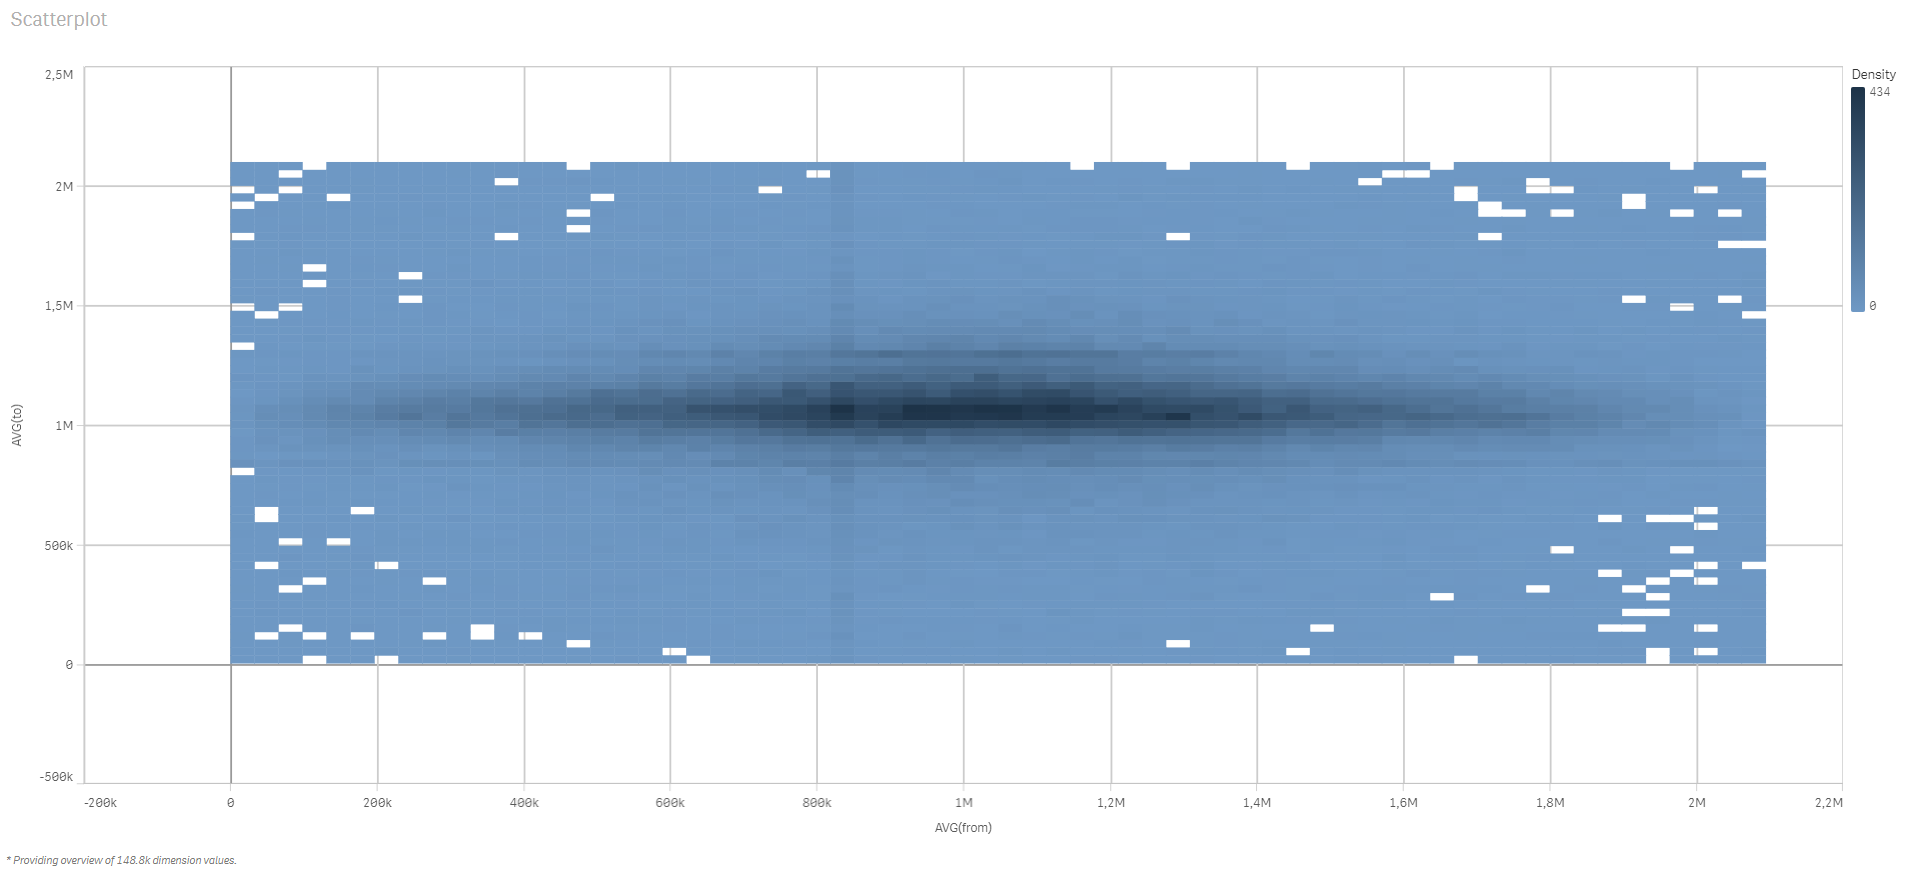
\includegraphics[width=6cm]{src/images/SmartDataCompression}}
    \caption{Smart Data Compression (left): Overview level which shows aggregated data points by squares and color and changes the shape if zoomed in}
    \label{fig:smartdatacompression}
\end{figure}

\begin{figure}[H]
    \centering
    \subfloat[Sparse Area]{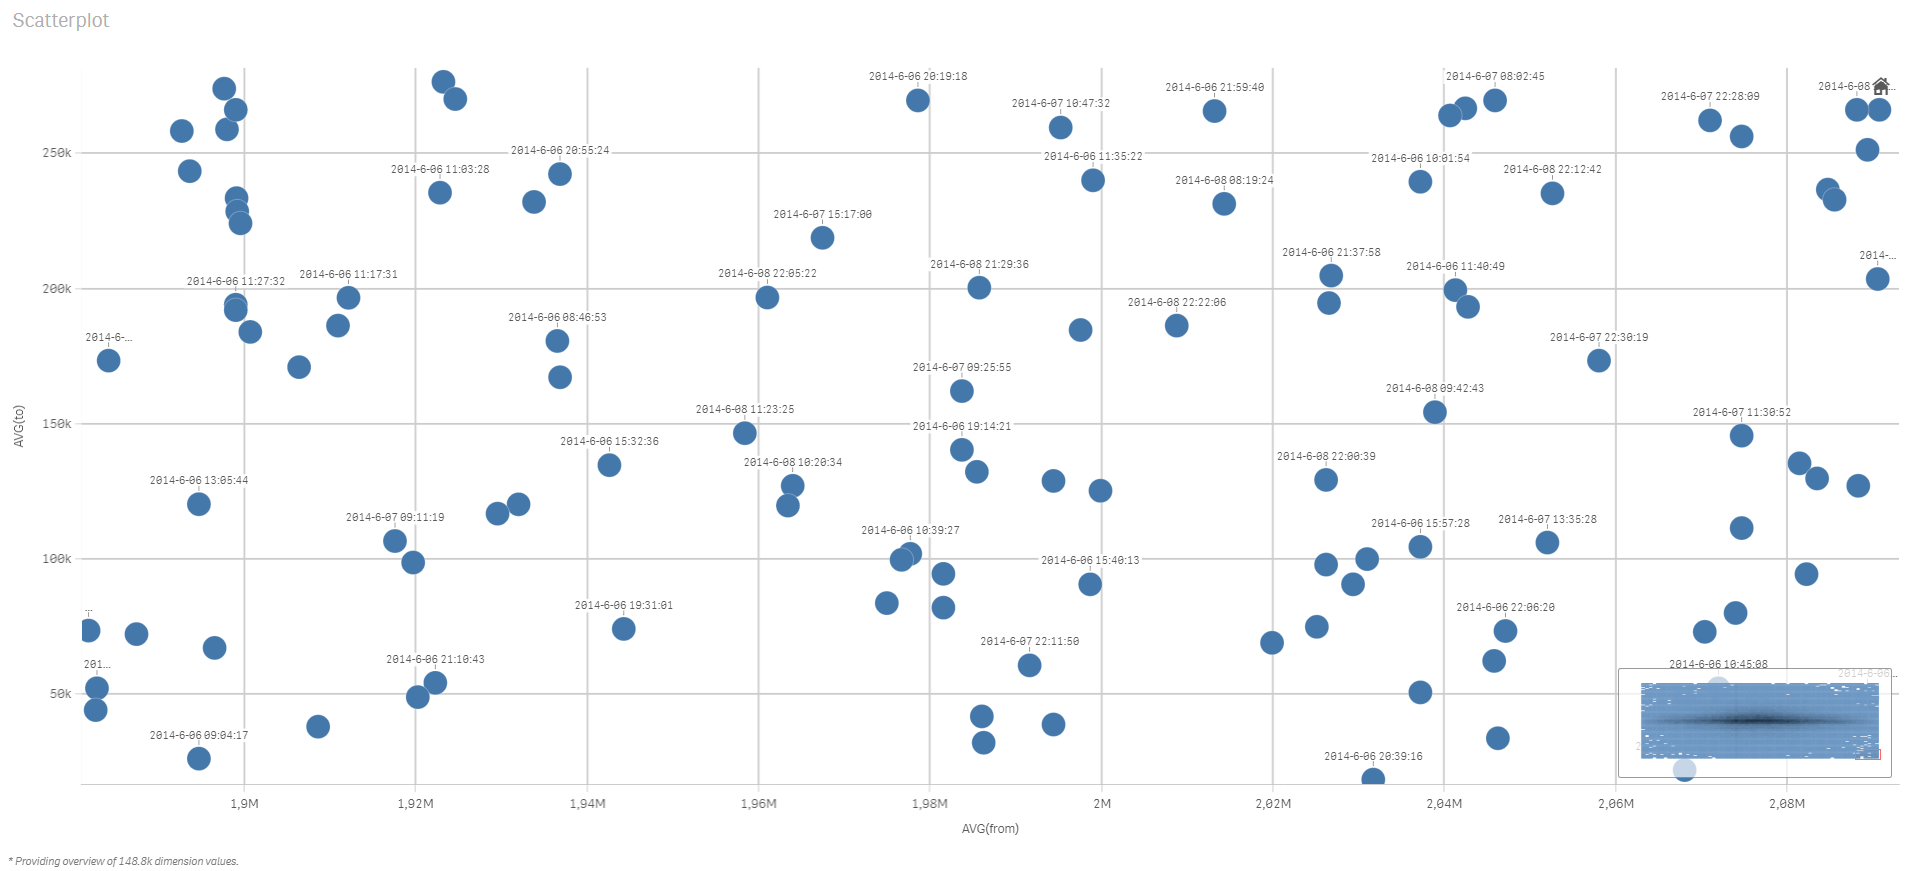
\includegraphics[width=6cm]{src/images/SmartDataCompressionI}}
    \qquad
    \subfloat[Dense Area]{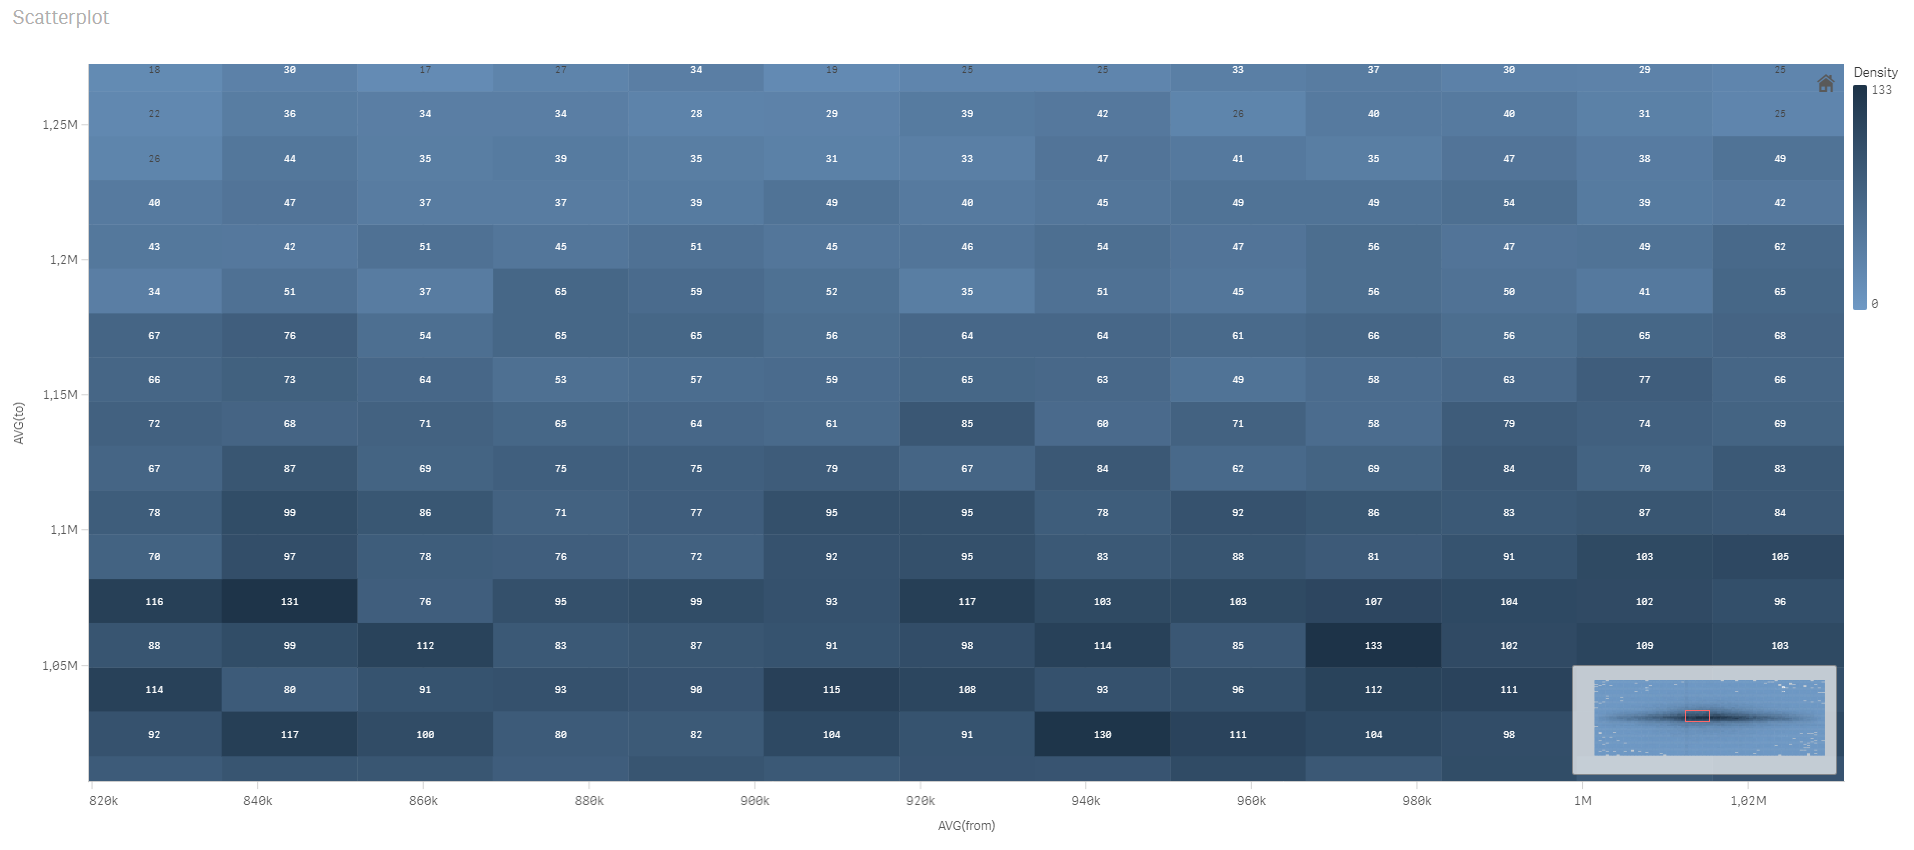
\includegraphics[width=6cm]{src/images/SmartDataCompressionII}}
    \caption{Smart Data Compression: Detail level}
    \label{fig:smartdatacompression}
\end{figure}

\textbf{Analytical Techniques}\\
Data reduction is part of QS Server. With dynamic data reduction (DDR) rows can be hidden for a group of users. Thus, data size is decreased. Internally, .QVD files compress data. But, the user cannot reduce data size based on an interactive selection inside the dashboard. 
%In this case, the user could select a group of data and decide whether he wants to keep only the selected data. 
QS implements \textbf{Aggregation} with aggregation-functions. These use QS specific set expressions (SE) and range from basic statistical functions (min,avg,max) over financial functions, to advanced statistical functions(linear regression, correlation). With these aggregation functions QS offers some analytical methods. Yet, QS has no integration to an analytical program.\\*

\textbf{Interaction Techniques}\\
QS offers mini charts (MiC) which are one implementation of navigational maps\cite{beard1990navigational}. Mini Charts come as a navigational slider in which a miniature version of the whole data set\cite{beard1990navigational} is shown. 
Filters can be applied by making selections or dragging a filter inside the visualization\cite{qlikSheet}. All views then are adapted to the current selection. Thus, QS offers Brushing + Linking. An additional linking-feature are \textit{master items}\cite{qlikChangeData}, which allow the user to change properties for all master items at once.
For details the user can search QS with Smart Search in which the dimensions, measures and metadata is searched and visualizations ,tables and KPIs are displayed\cite{qlikSmart}.  

\newpage
\todo{ggf newpage rausnehmen}
\subsection*{Tableau}

\textbf{Visualization Techniques}\\
Tableau offers 22 built-in visualization techniques: heat maps, symbol maps, stacked bars, pie charts, horizontal bars, side-by-side bars, treemaps, circle views, side-by-side circles, continuous lines, discrete lines, dual lines, area charts,  discrete area charts, dual combination, scatter plots, histogram, box-and-whisker plots, Gantt chart, bullet graphs and packed bubbles.
Visualization extensions are not possible even though Tableau has a JavaScript API. This API allows the integration of a Tableau dashboard into a web page, but is not built for writing JavaScript extensions for Tableau. Besides, advanced metahpors such as multi-resolution, data abstraction or aggregation markers are not supported. 
In sum, Tableau is a well-known choice in the visualization community. But it does not support large scale visualization features. \\*

\textbf{Analytical Techniques}\\
Tableau's analytical strength is manifested in the support of analytical functions. On the one hand, Tableau offers build-in modelling functions: prediction, trend line, cluster, average and median. Furthermore, R scripts can be loaded into Tableau.  
In terms of data reduction data extracts (DE) can be build based on the data connection. Therefore, filters can be applied and the data set reduced to the filtered data, unused columns can be hidden. 

\textbf{Interaction Techniques}\\
Regarding interaction Tableau offers Brushing\&Linking, Zooming and  \hyperlink{http://kb.tableau.com/articles/howto/adding-filters-to-dashboards}{Filtering}. Furthermore, Tableau supports Pan\& Zoom. 
Speaking of navigation techniques Tableau offers coordinated windows. 
Distortion techniques, Search and Navigational Sliders are not supported. 
\newpage
\subsection*{Power BI}

\textbf{Visualization Techniques}\\
Microsoft Power BI offers 8 built-in visualization techniques, 15 available techniques at the MarketPlace and 75 visualization apps in the visuals gallery. Additionally, the user can build custom visualization apps by writing \textit{TypeScript} or \textit{R}. Out of the 98 techniques none of them implements any discussed techniques of chapter \ref{chap:BIV}. Moreover, so far advanced Metaphors are not supported\cite{Amanda}. One approach to aggregation markers are \hyperlink{https://Power BI.microsoft.com/de-de/blog/power-bi-desktop-october-feature-summary/#grouping}{\textit{Groups}} which can be combined with drill-down options.\\*

\textbf{Analytical Techniques}\\
Data Reduction in Power BI is possible with a data view on the database (V) which considers less data than before. Moreover, data sets can be extracted (DE) with the \hyperlink{https://Power BI.microsoft.com/de-de/blog/power-bi-desktop-october-feature-summary/#grouping}{\textit{Inclusion/Exclusion}} of data points.\\*
\textit{Integration of analytical program:} Besides the own core functions for data reduction Power BI is connected to analytical programs such as \hyperlink{https://Power BI.microsoft.com/de-de/blog/power-bi-desktop-october-feature-summary/#grouping}{\textit{R, Mixpanel or comScore.}}\\*
\textit{Aggregation and Sampling} for example can be achieved in embedding R scripts or in using calculated fields. \\*

\textbf{Interaction Techniques}\\
With cross-highlighting Power BI includes brushing and linking\cite{Power BIInteract}. Moreover, filter functions are embedded. The \textit{focus mode} expands one visualization to full screen and thus, enables the user to have a detailed view on the visualization. The app \textit{Advanced Time Slicer} is one implementation of the navigation technique navigational map for time-oriented data. Navigation in Power BI is also realized by the search mechanism Power Q&A which answers NLP-question regarding the data set. Power Q&A includes filtering with the keywords WHERE, AFTER, BEFORE, BETWEEN, WITH or by naming the date as well. Besides the integrated navigation techniques other interactions can be embedded with visualization extensions (E) written in TypeScript.
\newpage
\subsection*{d3.js}
\textbf{Visualization Techniques}\\
In d3.js data attributes are assigned to graphical attributes. Thus, different way exist to visualize the same visualization technique. By writing JavaScript code any visualization technique any advanced metaphor can be implemented. Some examples are d3.hexbin which allows binning,  simplify.js for data abstraction or clusterfck for clustering.  
Marker clustering in d3.js for example can be achieved with \href{https://www.phase2technology.com/blog/using-d3-quadtrees-to-power-an-interactive-map-for-bonnier-corporation/}{quadtrees}\cite{Morrison2014}. Simplify.js for example reduces data points on polylines while maintaining the characteristic shape of the polyline. This is one example for data abstraction (DA).\\*

\textbf{Analytical Techniques}\\
While d3.js is only designed to visualize data it does not inherently offer the ability to analyze data. Therefore, a number of JavaScript libraries (L) exist which can be combined with d3.js. Some examples are simplestatistics.js, regression.js, node.js with the packages data-reduction, ml-pca or dimensionality-reduction. 
As JavaScript allows the integration of libraries there is no limit for analytical functions. \\*

\textbf{Interaction Techniques}\\
d3.js allows to integrate various interaction techniques such as Zooming, Filtering or Linking \& Brushing. Distortion techniques can be achieved with the d3 plugin \hyperlink{https://bost.ocks.org/mike/fisheye/}{\textit{Fisheye Distortion (FD)}}\cite{Bostock2012} which allows circular, linear and logarithmic distortion.
Perspective walls can be implemented with \hyperlink{https://bl.ocks.org/mbostock/10571478}{\textit{Perspective Transformation (PT) }}\cite{Bostock2017}.\\


\begin{table}[H]

    \begin{tabular}{|l| l l l l l|}
        \hline
        \multicolumn{2}{|c}{}   & d3.js  & QS  & Power BI & Tableau\\\hline
        \multirow{9}*{Analytics}
        & \multicolumn{5}{l|}{\cellcolor{gray!30} Horizontal Data Reduction}\\\cline{2-6}
        & Dimensionality Reduction & L, DA & \hyperlink{https://help.qlik.com/en-US/sense/1.0/Subsystems/WorkingWith/Content/ChartFunctions/SetAnalysis/AnalyzeSetsOfData.htm}{SE} & E & E \\\cline{2-6}
        & \multicolumn{5}{l|}{\cellcolor{gray!30}Vertical Data Reduction}\\\cline{2-6}
        %& Vertical Data Reduction           & L  &  DDR & DE,E,J,V    &   DE,E       \\ 
        & Sampling & L & DDR & J,V & DE,E\\
        & Filtering & L & DB & DE & DE\\
        & Aggregation & L & A & A & A \\
        & Abstraction & L & - & - & - \\\cline{2-6}
        &\rowcolor{gray!30}  Data Modeling & L  & -    & T,MM    & T, MM, F \\\cline{2-6}
        &\rowcolor{gray!30}  Pattern Search& L  & -    & -       & - \\
        \hline
        \multirow{3}*{Visualization}
        & ADV                       & P     & E    & E &-   \\
        & Multi-Resolution          & P     & E    & E & -  \\
        & Aggregation Markers       & MC    & SDC  & E & -  \\
        
        \hline
        \multirow{11}*{Interaction}
        
        & \multicolumn{5}{l|}{\cellcolor{gray!30}Standard Techniques}\\\cline{2-6}
        & Filter                & P & N & N & N \\
        & Zooming               & P & N & N & N \\ \cline{2-6}
        
        & \multicolumn{5}{l|}{\cellcolor{gray!30}Distortion Techniques}\\\cline{2-6}
        & Graphical Fish-eye    & \hyperlink{https://bost.ocks.org/mike/fisheye/}{FD}\cite{Bostock2012}       & E  & E  & - \\
        & Bifocal-Display       & \hyperlink{https://bost.ocks.org/mike/fisheye/}{FD}\cite{Bostock2012}       & E  & E  & - \\
        & Perspective Walls     & PT & E & E & - \\ \cline{2-6}
        
        & \multicolumn{5}{l|}{\cellcolor{gray!30}Navigation Techniques}\\\cline{2-6}
        & Brushing \& Linking   & P & N & N & N \\
        & Search                &  L & \hyperlink{https://help.qlik.com/en-US/sense/2.2/Subsystems/Hub/Content/Search/search-tool.htm}{SS}& \hyperlink{https://powerbi.microsoft.com/en-us/documentation/powerbi-service-q-and-a/}{Q\&A}& - \\
        & Navigational Maps     & P & \hyperlink{https://help.qlik.com/en-US/sense/1.1/Subsystems/Hub/Content/Visualizations/BarChart/BarChart.htm}{MiC}  & -           & -\\
        \hline
    \end{tabular}
    \caption{Overview of Tool Comparison}
    \end{table}
    
    Analytics\\*
    L = Library, DA = Data Abstraction, DDR = Dynamic Data Reduction, DE = Data Extraction, E = Extensions, F = Forecasting, J = Joins, MM = Min-Max-Function, SE = Set Expressions, T = Trendline, V = Views, - = not existing
    \par 
    Visualization\\*
    P = Programmable, E = Extensions, MC = Marker Clustering, SDC = Smart Data Compression, - = not existing
    \par
    Interaction\\*
    E = Extensions, FD = Fisheye Distortion, MiC = Mini Charts, N = Natively Integrated, P = Programmable, PT = Perspective Tranformation, Q\&A = Question \& Answer,  SS = Smart Search, - = not existing
 
\begin{table}[H]

    \begin{tabular}{|l| l l l l l|}
        \hline
        \multicolumn{2}{|c}{}   & d3.js  & QS  & Power BI & Tableau\\\hline
        \multirow{9}*{Analytics}
        & \multicolumn{5}{l|}{\cellcolor{gray!30} Horizontal Data Reduction}\\\cline{2-6}
        
        & Dimensionality Reduction & 3,2 & 4,1 & 3,2 & 3,2  \\\cline{2-6}
        & \multicolumn{5}{l|}{\cellcolor{gray!30}Vertical Data Reduction}\\\cline{2-6}
        & Sampling & 3,2 & 3,2 & 1,1/ 3,2 & 1,1/ 3,2 \\
        & Filtering & 3,2 & 0/ 1,2 & 1,2/3,2 & 1,1/ 2,2\\
        & Aggregation & 3,2 & 4,2 & 1,2 & 1,2 \\
        & Abstraction & 3,2 & 0 & 0 & 0\\\cline{2-6}
        &\rowcolor{gray!30} Integration to analytical program & 3,2 & 0 & 3,2 & 3,2  \\\cline{2-6}
        &\rowcolor{gray!30} Data Modeling  & 3,2 & 4,1 & 2,1/ 3,2 & 1.5,2/ 3,2 \\\cline{2-6}
        &\rowcolor{gray!30} Pattern Search & 3,2 & 0 &  0  & 0\\
        \hline
        \multirow{3}*{Visualization}
        & ADV                   &   3,2  &  4,2 & 4,2 & 0  \\
        & Aggregation Markers   &   3,2  &  1,1/4,2 & 4,2 &  0 \\
        & Multi-Resolution      &   3,2  &  4,2 & 4,2 & 0  \\
        
        \hline
        \multirow{11}*{Interaction}
        
        & \multicolumn{5}{l|}{\cellcolor{gray!30}Standard Techniques}\\\cline{2-6}
        & Filter                & 3,2 & 1.5,2 & 1.5,2 & 1.5,2 \\
        & Zooming               & 3,2 & 1,2 & 1,2 & 1,2 \\ \cline{2-6}
        
        & \multicolumn{5}{l|}{\cellcolor{gray!30}Distortion Techniques}\\\cline{2-6}
        & Graphical Fish-eye    & 3,2 & 4,2 & 4,2 & 0 \\
        & Bifocal-Display       & 3,2 & 4,2 & 4,2 & 0 \\
        & Perspective Walls     & 3,2 & 4,2 & 4,2 & 0 \\ \cline{2-6}
        
        & \multicolumn{5}{l|}{\cellcolor{gray!30}Navigation Techniques}\\\cline{2-6}
        & Brushing \& Linking   & 3,2 & 1,2 & 1,2 & 1,2\\
        & Search                & 3,2 & 1,2 & 1,2 & 0 \\
        & Navigational Maps     & 3,2 & 1,2 & 1,1 & 0 \\
        \hline
    \end{tabular}
    \caption{Tool Comparison with Scoring based on the degree of implementation}
    \end{table}
   
\subsection*{TCS of Analytical Techniques}
The TCS has been determined for different aspects of \textit{Support of Analytical Techniques} and \textit{Integration of Analytical Program}. Both aspects are relevant for horizontal and vertical data reduction. Therefore, a tool either can offer data reduction techniques by itself or it can integrate an analytical program such as R. Built-in-functions require less programming skills while the integration of an analytical program usually offers a wider spectrum of data reduction techniques.
Among the assessed analytical technique are sampling, filtering, data abstraction and  dimensionality reduction.

%%% Horizontal Data Reduction
\begin{figure}[H]
\subfigure[Dimensionality Reduction]
{
    \begin{tikzpicture}[scale=0.55]
        \begin{axis}[
        axis y line     = left,
        axis x line     = bottom,
        grid,
        grid style = {color=gray!50, dotted},
        width = 10cm, 
        height = 5cm,
        xticklabels={,,1,2,3,4},
        yticklabels={,0,1,2},
        xmin       = -0.1, domain = 0:4, xmax = 4.5,
        ymin       = -0.1, domain = 0:2, ymax = 2.5,
        xlabel={Programming-Skills},ylabel={Completeness}
        ]
        % (1) Supports Analytical Functions
         \addplot [] coordinates{};
        \node[rectangle with four colors, top color=d3orange, right color=yellow, bottom color=yellow, left color=blue!50,
        draw]  at (axis cs: 3,2) {}; %d3.js
        \node[rectangle with four colors, top color=applegreen, right color=applegreen, bottom color=applegreen, left color=applegreen,
        draw]  at (axis cs: 4,1) {}; %QS, Power BI, Tableau
        % \node[rectangle with four colors, top color=yellow, right color=yellow, bottom color=yellow, left color=yellow,
        % draw]  at (axis cs: 1,1) {}; %Power BI
        % \node[rectangle with four colors, top color=blue!50, right color=blue!50, bottom color=blue!50, left color=blue!50,
        % draw]  at (axis cs: 1,1) {}; %Tableau
        % \node[rectangle with four colors, top color=blue!50, right color=blue!50, bottom color=blue!50, left color=blue!50,
        % draw]  at (axis cs: 4,1) {}; %Tableau
        \end{axis}
    \end{tikzpicture}
}    
\subfigure[Integration of Analytical program]
{  
    \begin{tikzpicture}[scale=0.55]
        \begin{axis}[
        axis y line     = left,
        axis x line     = bottom,
        grid,
        grid style = {color=gray!50, dotted},
        width = 10cm, 
        height = 5cm,
        xticklabels={,,1,2,3,4},
        yticklabels={,0,1,2},
        xmin       = -0.1, domain = 0:4, xmax = 4.5,
        ymin       = -0.1, domain = 0:2, ymax = 2.5,
        xlabel={Programming-Skills},ylabel={Completeness}
        ]
        % (2) Integration with analytical program
        \addplot [] coordinates{};
        \node[rectangle with four colors, top color=d3orange, right color=yellow, bottom color=yellow, left color=blue!50,
        draw]  at (axis cs: 3,2) {}; %d3.js, Tableau, Power BI
        \node[rectangle with four colors, top color=applegreen, right color=applegreen, bottom color=applegreen, left color=applegreen,
        draw]  at (axis cs: 0,0) {}; %QS
        \end{axis}
        \begin{customlegend}[
            legend entries={ % <= in the following there are the entries
                d3.js,
                Power BI,
                QS,
                Tableau
            },
            legend style={at={(13.5, 3.5)},font=\footnotesize}] % <= to define position and font legend
            % the following are the "images" and numbers in the legend
            \addlegendimage{mark=*,d3orange,opacity=1}
            \addlegendimage{mark=*,yellow,opacity=0.5}
            \addlegendimage{mark=*,applegreen,opacity=1}
            \addlegendimage{mark=*,blue,opacity=0.5}
        \end{customlegend}
    \end{tikzpicture}
}
\caption{TCS regarding Horizontal Data Reduction} \label{TCShorizontal}
\end{figure}

%%%%%%%%%%% Vertical Data Reduction
\begin{figure}[H]
\subfigure[Sampling]
{
    \begin{tikzpicture}[scale=0.55]
        \begin{axis}[
        axis y line     = left,
        axis x line     = bottom,
        grid,
        grid style = {color=gray!50, dotted},
        width = 10cm, 
        height = 5cm,
        xticklabels={,,1,2,3,4},
        yticklabels={,0,1,2},
        xmin       = -0.1, domain = 0:4, xmax = 4.5,
        ymin       = -0.1, domain = 0:2, ymax = 2.5,
        xlabel={Programming-Skills},ylabel={Completeness}
        ]
        % (1) Sampling
        \addplot [] coordinates{};
        \node[rectangle with four colors, top color=d3orange, right color=yellow, bottom color=blue!50, left color=applegreen,
        draw]  at (axis cs: 3,2) {}; %d3.js, Power BI, Tableau, QS
        \node[rectangle with four colors, top color=yellow, right color=yellow, bottom color=blue!50, left color=blue!50,
        draw]  at (axis cs: 0,0) {}; %Power BI, Tableau
        \end{axis}
    \end{tikzpicture}
}    
\subfigure[Filtering]
{  
    \begin{tikzpicture}[scale=0.55]
        \begin{axis}[
        axis y line     = left,
        axis x line     = bottom,
        grid,
        grid style = {color=gray!50, dotted},
        width = 10cm, 
        height = 5cm,
        xticklabels={,,1,2,3,4},
        yticklabels={,0,1,2},
        xmin       = -0.1, domain = 0:4, xmax = 4.5,
        ymin       = -0.1, domain = 0:2, ymax = 2.5,
        xlabel={Programming-Skills},ylabel={Completeness}
        ]
        % (2) Filtering
        \addplot [] coordinates{};
        \node[rectangle with four colors, top color=applegreen, right color=applegreen, bottom color=yellow, left color=yellow,
        draw]  at (axis cs: 3,2) {}; %QS, Power BI
        \node[rectangle with four colors, top color=d3orange, right color=d3orange, bottom color=yellow, left color=yellow,
        draw]  at (axis cs: 3,2) {}; %d3.js, Power BI
        \node[rectangle with four colors, top color=applegreen, right color=applegreen, bottom color=applegreen, left color=applegreen,
        draw]  at (axis cs: 0,0) {}; %QS
        \node[rectangle with four colors, top color=blue!50, right color=blue!50, bottom color=blue!50, left color=blue!50,
        draw]  at (axis cs: 1,1) {}; %Tableau
        \end{axis}
    \end{tikzpicture}
}

% \subfigure[Filtering + Extraction]
% {  
%     \begin{tikzpicture}[scale=0.55]
%         \begin{axis}[
%         axis y line     = left,
%         axis x line     = bottom,
%         grid,
%         grid style = {color=gray!50, dotted},
%         width = 10cm, 
%         height = 5cm,
%         xticklabels={,,1,2,3,4},
%         yticklabels={,0,1,2},
%         xmin       = -0.1, domain = 0:4, xmax = 4.5,
%         ymin       = -0.1, domain = 0:2, ymax = 2.5,
%         xlabel={Programming-Skills},ylabel={Completeness}
%         ]
%         % (2) Filtering + Extraction
%         \addplot [] coordinates{};
%         \node[rectangle with four colors, top color=d3orange, right color=d3orange, bottom color=d3orange, left color=d3orange,
%         draw]  at (axis cs: 3,4) {}; %d3.js
%         \node[rectangle with four colors, top color=applegreen, right color=applegreen, bottom color=applegreen, left color=applegreen,
%         draw]  at (axis cs: 0,0) {}; %QS
%         \node[rectangle with four colors, top color=yellow, right color=yellow, bottom color=yellow, left color=yellow,
%         draw]  at (axis cs: 1,4) {}; %Power BI
%         \node[rectangle with four colors, top color=blue!50, right color=blue!50, bottom color=blue!50, left color=blue!50,
%         draw]  at (axis cs: 2,4) {}; %Tableau
%         \end{axis}
%     \end{tikzpicture}
% }
\subfigure[Aggregation]
{  
    \begin{tikzpicture}[scale=0.55]
        \begin{axis}[
        axis y line     = left,
        axis x line     = bottom,
        grid,
        grid style = {color=gray!50, dotted},
        width = 10cm, 
        height = 5cm,
        xticklabels={,,1,2,3,4},
        yticklabels={,0,1,2},
        xmin       = -0.1, domain = 0:4, xmax = 4.5,
        ymin       = -0.1, domain = 0:2, ymax = 2.5,
        xlabel={Programming-Skills},ylabel={Completeness}
        ]
        % (2) Aggregation
        \addplot [] coordinates{};
        \node[rectangle with four colors, top color=d3orange, right color=d3orange, bottom color=d3orange, left color=d3orange,
        draw]  at (axis cs: 3,2) {}; %d3.js
        \node[rectangle with four colors, top color=applegreen, right color=applegreen, bottom color=applegreen, left color=applegreen,
        draw]  at (axis cs: 4,2) {}; %QS
        \node[rectangle with four colors, top color=yellow, right color=yellow, bottom color=blue!50, left color=blue!50,
        draw]  at (axis cs: 1,2) {}; %Power BI, Tableau
        \end{axis}
    \end{tikzpicture}
}
\subfigure[Abstraction]
{
\begin{tikzpicture}[scale=0.55]
        \begin{axis}[
        axis y line     = left,
        axis x line     = bottom,
        grid,
        grid style = {color=gray!50, dotted},
        width = 10cm, 
        height = 5cm,
        xticklabels={,,1,2,3,4},
        yticklabels={,0,1,2},
        xmin       = -0.1, domain = 0:4, xmax = 4.5,
        ymin       = -0.1, domain = 0:2, ymax = 2.5,
        xlabel={Programming-Skills},ylabel={Completeness}
        ]
        % (3) Abstraction
         \addplot [] coordinates{};
        \node[rectangle with four colors, top color=d3orange, right color=d3orange, bottom color=d3orange, left color=d3orange,
        draw]  at (axis cs: 3,2) {}; %d3.js
       \node[rectangle with four colors, top color=applegreen, right color=blue!50, bottom color=yellow, left color=white,
        draw]  at (axis cs: 0,0) {}; %QS, Power BI, Tableau
        \end{axis}
    \end{tikzpicture}
}
\caption{TCS regarding Vertical Data Reduction} \label{TCSvertical}
\end{figure}

%%%% Data Modeling
\begin{figure}[H]
    \begin{tikzpicture}[scale=0.55]
        \begin{axis}[
        axis y line     = left,
        axis x line     = bottom,
        grid,
        grid style = {color=gray!50, dotted},
        width = 10cm, 
        height = 5cm,
        xticklabels={,,1,2,3,4},
        yticklabels={,0,1,2},
        xmin       = -0.1, domain = 0:4, xmax = 4.5,
        ymin       = -0.1, domain = 0:2, ymax = 2.5,
        xlabel={Programming-Skills},ylabel={Completeness}
        ]
        \addplot [] coordinates{};
        \node[rectangle with four colors, top color=d3orange, right color=yellow, bottom color=blue!50, left color=blue!50,
        draw]  at (axis cs: 3,2) {}; %d3.js
        \node[rectangle with four colors, top color=applegreen, right color=applegreen, bottom color=applegreen, left color=applegreen,
        draw]  at (axis cs: 4,1) {}; %QS
        \node[rectangle with four colors, top color=yellow, right color=yellow, bottom color=yellow, left color=yellow,
        draw]  at (axis cs: 2,1) {}; %Power BI
        \node[rectangle with four colors, top color=blue!50, right color=blue!50, bottom color=blue!50, left color=blue!50,
        draw]  at (axis cs: 1.5,2) {}; %Tableau    
        \end{axis}
    \end{tikzpicture}
\caption{TCS regarding Data Modeling} \label{TCSdataModeling}
\end{figure}
%%% Pattern Search
\begin{figure}[H]
    \begin{tikzpicture}[scale=0.55]
        \begin{axis}[
        axis y line     = left,
        axis x line     = bottom,
        grid,
        grid style = {color=gray!50, dotted},
        width = 10cm, 
        height = 5cm,
        xticklabels={,,1,2,3,4},
        yticklabels={,0,1,2},
        xmin       = -0.1, domain = 0:4, xmax = 4.5,
        ymin       = -0.1, domain = 0:2, ymax = 2.5,
        xlabel={Programming-Skills},ylabel={Completeness}
        ]
        \addplot [] coordinates{};
        \node[rectangle with four colors, top color=d3orange, right color=d3orange, bottom color=d3orange, left color=d3orange,
        draw]  at (axis cs: 3,2) {}; %d3.js
       \node[rectangle with four colors, top color=applegreen, right color=blue!50, bottom color=yellow, left color=white,
        draw]  at (axis cs: 0,0) {}; %QS, Power BI, Tableau
        \end{axis}
    \end{tikzpicture}
\caption{TCS regarding Pattern Search} \label{TCSpatternSearch}
\end{figure}

\subsection*{Visualization}
The TCS of Visualization covers the support of advanced visualization techniques and the support of advanced visual metaphors. Techniques either can be natively integrated or achieved by programming an extension. Therefore, one aspect is \textit{Extendability}. Among advanced visual metaphors \textit{Aggregation Markers} and \textit{Multi-Resolution} has been assessed.
\begin{figure}[H]
\subfigure[Support of ADV]
{
    \begin{tikzpicture}[scale=0.55]
        \begin{axis}[
        axis y line     = left,
        axis x line     = bottom,
        grid,
        grid style = {color=gray!50, dotted},
        width = 10cm, 
        height = 5cm,
        xticklabels={,,1,2,3,4},
        yticklabels={,0,1,2},
        xmin       = -0.1, domain = 0:4, xmax = 4.5,
        ymin       = -0.1, domain = 0:2, ymax = 2.5,
        xlabel={Programming-Skills},ylabel={Completeness}
        ]
        % (1) Offers advanced techniques
        \addplot [] coordinates{};
        \node[rectangle with four colors, top color=d3orange, right color=d3orange, bottom color=d3orange, left color=d3orange,
        draw]  at (axis cs: 3,2) {}; %d3.js
        \node[rectangle with four colors, top color=applegreen, right color=applegreen, bottom color=yellow, left color=yellow,
        draw]  at (axis cs: 4,2) {}; %QS, Power BI
        \node[rectangle with four colors, top color=blue!50, right color=blue!50, bottom color=blue!50, left color=blue!50,
        draw]  at (axis cs: 0,0) {}; %Tableau
        \end{axis}
    \end{tikzpicture}
}
\subfigure[Aggregation Marker]
{  
    \begin{tikzpicture}[scale=0.55]
        \begin{axis}[
        axis y line     = left,
        axis x line     = bottom,
        grid,
        grid style = {color=gray!50, dotted},
        width = 10cm, 
        height = 5cm,
        xticklabels={,,1,2,3,4},
        yticklabels={,0,1,2},
        xmin       = -0.1, domain = 0:4, xmax = 4.5,
        ymin       = -0.1, domain = 0:2, ymax = 2.5,
        xlabel={Programming-Skills},ylabel={Completeness}
        ]
        % (2) Aggregation Markers
        \addplot [] coordinates{};
        \node[rectangle with four colors, top color=d3orange, right color=d3orange, bottom color=d3orange, left color=d3orange,
        draw]  at (axis cs: 3,2) {}; %d3.js
        \node[rectangle with four colors, top color=applegreen, right color=applegreen, bottom color=applegreen, left color=applegreen,
        draw]  at (axis cs: 1,1) {SDC}; %QS
        \node[rectangle with four colors, top color=applegreen, right color=applegreen, bottom color=yellow, left color=yellow,
        draw]  at (axis cs: 4,2) {}; %QS, Power BI
        \node[rectangle with four colors, top color=blue!50, right color=blue!50, bottom color=blue!50, left color=blue!50,
        draw]  at (axis cs: 0,0) {}; %Tableau

        
        \end{axis}
    \end{tikzpicture}
}

\subfigure[Multi-resolution]
{
\begin{tikzpicture}[scale=0.55]
        \begin{axis}[
        axis y line     = left,
        axis x line     = bottom,
        grid,
        grid style = {color=gray!50, dotted},
        width = 10cm, 
        height = 5cm,
        xticklabels={,,1,2,3,4},
        yticklabels={,0,1,2},
        xmin       = -0.1, domain = 0:4, xmax = 4.5,
        ymin       = -0.1, domain = 0:2, ymax = 2.5,
        xlabel={Programming-Skills},ylabel={Completeness}
        ]
        % (3) Multi-Resolution Metaphor
        \addplot [] coordinates{};
        \node[rectangle with four colors, top color=d3orange, right color=d3orange, bottom color=d3orange, left color=d3orange,
        draw]  at (axis cs: 3,2) {}; %d3.js
        \node[rectangle with four colors, top color=applegreen, right color=applegreen, bottom color=yellow!50, left color=yellow,
        draw]  at (axis cs: 4,2) {}; %QS, Power BI
        \node[rectangle with four colors, top color=blue!50, right color=blue!50, bottom color=blue!50, left color=blue!50,
        draw]  at (axis cs: 0,0) {}; %Tableau
        \end{axis}
    \end{tikzpicture}
}

\caption{TCS regarding Visualization: similar positioning of tools across all criteria} \label{TCSvisualization}
\end{figure}

\textbf{Interaction Techniques}\\
The TCS of Interaction Techniques includes standard interaction techniques such as \textit{Brushing \& Linking, Zooming and Filtering}. In contrast to analytical techniques filtering does not reduce the actual data size but only the selected values. \textit{Distortion Techniques} has been assessed as well as \textit{Coordinated Windows, Search and Navigational Maps} among the navigation techniques. 
%%% Standard Interaction
\begin{figure}[H]

\subfigure[Filter]
{
\begin{tikzpicture}[scale=0.55]
        \begin{axis}[
        axis y line     = left,
        axis x line     = bottom,
        grid,
        grid style = {color=gray!50, dotted},
        width = 10cm, 
        height = 5cm,
        xticklabels={,,1,2,3,4},
        yticklabels={,0,1,2},
        xmin       = -0.1, domain = 0:4, xmax = 4.5,
        ymin       = -0.1, domain = 0:2, ymax = 2.5,
        xlabel={Programming-Skills},ylabel={Completeness}
        ]
        % (1) Filter
        \addplot [] coordinates{};
        \node[rectangle with four colors, top color=d3orange, right color=d3orange, bottom color=d3orange, left color=d3orange,
        draw]  at (axis cs: 3,2) {}; %d3.js
       \node[rectangle with four colors, top color=applegreen, right color=blue!50, bottom color=yellow, left color=white,
        draw]  at (axis cs: 1.5,2) {}; %QS, Power BI, Tableau
        \end{axis}
    \end{tikzpicture}
}
\subfigure[Zoom]
{  
    \begin{tikzpicture}[scale=0.55]
        \begin{axis}[
        axis y line     = left,
        axis x line     = bottom,
        grid,
        grid style = {color=gray!50, dotted},
        width = 10cm, 
        height = 5cm,
        xticklabels={,,1,2,3,4},
        yticklabels={,0,1,2},
        xmin       = -0.1, domain = 0:4, xmax = 4.5,
        ymin       = -0.1, domain = 0:2, ymax = 2.5,
        xlabel={Programming-Skills},ylabel={Completeness}
        ]
        % (2) Zoom
        \addplot [] coordinates{};
        \node[rectangle with four colors, top color=d3orange, right color=d3orange, bottom color=d3orange, left color=d3orange,
        draw]  at (axis cs: 3,2) {}; %d3.js
       \node[rectangle with four colors, top color=applegreen, right color=blue!50, bottom color=yellow, left color=white,
        draw]  at (axis cs: 1,2) {}; %QS, Power BI, Tableau
        \end{axis}
    \end{tikzpicture}
}
\caption{TCS regarding Standard Interaction Techniques: similar positioning of tools across all criteria} \label{TCSstandardinteraction}

\end{figure}

%% Distortion Techniques
\begin{figure}[H]
\subfigure[Graphical Fish-Eye]
{
    \begin{tikzpicture}[scale=0.55]
        \begin{axis}[
        axis y line     = left,
        axis x line     = bottom,
        grid,
        grid style = {color=gray!50, dotted},
        width = 10cm, 
        height = 5cm,
        xticklabels={,,1,2,3,4},
        yticklabels={,0,1,2},
        xmin       = -0.1, domain = 0:4, xmax = 4.5,
        ymin       = -0.1, domain = 0:2, ymax = 2.5,
        xlabel={Programming-Skills},ylabel={Completeness}
        ]
        % (1) Graphical Fish-Eye
        \addplot [] coordinates{};
        \node[rectangle with four colors, top color=d3orange, right color=d3orange, bottom color=d3orange, left color=d3orange,
        draw]  at (axis cs: 3,2) {}; %d3.js
       \node[rectangle with four colors, top color=applegreen, right color=applegreen, bottom color=yellow, left color=yellow,
        draw]  at (axis cs: 4,2) {}; %QS, Power BI
        \node[rectangle with four colors, top color=blue!50, right color=blue!50, bottom color=blue!50, left color=blue!50,
        draw]  at (axis cs: 0,0) {}; %Tableau
        \end{axis}
    \end{tikzpicture}
}    
\subfigure[Bifocal-Display]
{  
    \begin{tikzpicture}[scale=0.55]
        \begin{axis}[
        axis y line     = left,
        axis x line     = bottom,
        grid,
        grid style = {color=gray!50, dotted},
        width = 10cm, 
        height = 5cm,
        xticklabels={,,1,2,3,4},
        yticklabels={,0,1,2},
        xmin       = -0.1, domain = 0:4, xmax = 4.5,
        ymin       = -0.1, domain = 0:2, ymax = 2.5,
        xlabel={Programming-Skills},ylabel={Completeness}
        ]
        % (2) Bifocal-Display
        \addplot [] coordinates{};
        \node[rectangle with four colors, top color=d3orange, right color=d3orange, bottom color=d3orange, left color=d3orange,
        draw]  at (axis cs: 3,2) {}; %d3.js
        \node[rectangle with four colors, top color=applegreen, right color=applegreen, bottom color=yellow, left color=yellow,
        draw]  at (axis cs: 4,2) {}; %QS, Power BI
        \node[rectangle with four colors, top color=blue!50, right color=blue!50, bottom color=blue!50, left color=blue!50,
        draw]  at (axis cs: 0,0) {}; %Tableau
        \end{axis}
    \end{tikzpicture}
}

\subfigure[Perspective Wall]
{
\begin{tikzpicture}[scale=0.55]
        \begin{axis}[
        axis y line     = left,
        axis x line     = bottom,
        grid,
        grid style = {color=gray!50, dotted},
        width = 10cm, 
        height = 5cm,
        xticklabels={,,1,2,3,4},
        yticklabels={,0,1,2},
        xmin       = -0.1, domain = 0:4, xmax = 4.5,
        ymin       = -0.1, domain = 0:2, ymax = 2.5,
        xlabel={Programming-Skills},ylabel={Completeness}
        ]
        % (3) Perspective Wall
         \addplot [] coordinates{};
        \node[rectangle with four colors, top color=d3orange, right color=d3orange, bottom color=d3orange, left color=d3orange,
        draw]  at (axis cs: 3,2) {}; %d3.js
        \node[rectangle with four colors, top color=applegreen, right color=applegreen, bottom color=yellow, left color=yellow,
        draw]  at (axis cs: 4,2) {}; %QS, Power BI
        \node[rectangle with four colors, top color=blue!50, right color=blue!50, bottom color=blue!50, left color=blue!50,
        draw]  at (axis cs: 0,0) {}; %Tableau
        \end{axis}
    \end{tikzpicture}
}

\caption{TCS regarding Distortion Techniques: Tableau is outperformed} \label{TCSdistortion}
\end{figure}

%% Navigation Techniques
\begin{figure}[H]
\subfigure[Brushing \& Linking]
{
    \begin{tikzpicture}[scale=0.55]
        \begin{axis}[
        axis y line     = left,
        axis x line     = bottom,
        grid,
        grid style = {color=gray!50, dotted},
        width = 10cm, 
        height = 5cm,
        xticklabels={,,1,2,3,4},
        yticklabels={,0,1,2},
        xmin       = -0.1, domain = 0:4, xmax = 4.5,
        ymin       = -0.1, domain = 0:2, ymax = 2.5,
        xlabel={Programming-Skills},ylabel={Completeness}
        ]
        % (1) Brushing \& Linking
        \addplot [] coordinates{};
        \node[rectangle with four colors, top color=d3orange, right color=d3orange, bottom color=d3orange, left color=d3orange,
        draw]  at (axis cs: 3,2) {}; %d3.js
       \node[rectangle with four colors, top color=applegreen, right color=blue!50, bottom color=yellow, left color=white,
        draw]  at (axis cs: 1,2) {}; %QS, Power BI, Tableau
        \end{axis}
    \end{tikzpicture}
}    
\subfigure[Navigational Maps]
{  
    \begin{tikzpicture}[scale=0.55]
        \begin{axis}[
        axis y line     = left,
        axis x line     = bottom,
        grid,
        grid style = {color=gray!50, dotted},
        width = 10cm, 
        height = 5cm,
        xticklabels={,,1,2,3,4},
        yticklabels={,0,1,2},
        xmin       = -0.1, domain = 0:4, xmax = 4.5,
        ymin       = -0.1, domain = 0:2, ymax = 2.5,
        xlabel={Programming-Skills},ylabel={Completeness}
        ]
        % (2) Bifocal-Display
        \addplot [] coordinates{};
        \node[rectangle with four colors, top color=d3orange, right color=d3orange, bottom color=d3orange, left color=d3orange,
        draw]  at (axis cs: 3,2) {}; %d3.js
        \node[rectangle with four colors, top color=applegreen, right color=applegreen, bottom color=applegreen, left color=applegreen,
        draw]  at (axis cs: 1,2) {}; %QS
        \node[rectangle with four colors, top color=yellow, right color=yellow, bottom color=yellow, left color=yellow,
        draw]  at (axis cs: 1,1) {}; %Power BI
        \node[rectangle with four colors, top color=blue!50, right color=blue!50, bottom color=blue!50, left color=blue!50,
        draw]  at (axis cs: 0,0) {}; %Tableau
        \end{axis}
    \end{tikzpicture}
}

\subfigure[Search]
{
\begin{tikzpicture}[scale=0.55]
        \begin{axis}[
        axis y line     = left,
        axis x line     = bottom,
        grid,
        grid style = {color=gray!50, dotted},
        width = 10cm, 
        height = 5cm,
        xticklabels={,,1,2,3,4},
        yticklabels={,0,1,2},
        xmin       = -0.1, domain = 0:4, xmax = 4.5,
        ymin       = -0.1, domain = 0:2, ymax = 2.5,
        xlabel={Programming-Skills},ylabel={Completeness}
        ]
        % (3) Search
         \addplot [] coordinates{};
        \node[rectangle with four colors, top color=d3orange, right color=d3orange, bottom color=d3orange, left color=d3orange,
        draw]  at (axis cs: 3,2) {}; %d3.js
        \node[rectangle with four colors, top color=applegreen, right color=applegreen, bottom color=yellow, left color=yellow,
        draw]  at (axis cs: 1,2) {}; %QS, Power BI
        \node[rectangle with four colors, top color=blue!50, right color=blue!50, bottom color=blue!50, left color=blue!50,
        draw]  at (axis cs: 0,0) {}; %Tableau
        \end{axis}
    \end{tikzpicture}
}

\caption{TCS regarding Navigation Techniques} \label{TCSnavigation}
\end{figure}


% \subfigure[Coordinated Windows]
% {
%     \begin{tikzpicture}[scale=0.55]
%         \begin{axis}[
%         axis y line     = left,
%         axis x line     = bottom,
%         grid,
%         grid style = {color=gray!50, dotted},
%         width = 10cm, 
%         height = 5cm,
%         xticklabels={,,1,2,3,4},
%         yticklabels={,0,1,2},
%         xmin       = -0.1, domain = 0:4, xmax = 4.5,
%         ymin       = -0.1, domain = 0:2, ymax = 2.5,
%         xlabel={Programming-Skills},ylabel={Completeness}
%         ]
%         % (1) Coordinated Windows
%         \addplot [] coordinates{};
%         \node[rectangle with four colors, top color=d3orange, right color=d3orange, bottom color=d3orange, left color=d3orange,
%         draw]  at (axis cs: 3,4) {}; %d3.js
%       \node[rectangle with four colors, top color=applegreen, right color=blue!50, bottom color=yellow, left color=white,
%         draw]  at (axis cs: 1,4) {}; %QS, Power BI, Tableau
%         \end{axis}
%     \end{tikzpicture}
% }    



\subsubsection{Conclusion}\label{conclusion}
The tool comparison demonstrates that there exists different strategies for large data visualization. Moreover, while some tools already started to offer analytical, visualization and interaction techniques for large scale data there are still features which are not provided by any tool and thus, out of the studied tools none of the tools is currently suitable for the visual exploration of large data.\\
\textbf{Database Metrics}\\*
\todo{Text einfügen}
\par
\textbf{Analytics}\\*
Tableau's strength is the analytical data visualization with a focus of \textit{data preprocessing}. The integration of R and built-in-functions such as clustering and prediction support both \textit{data reduction} techniques and time-oriented user tasks. Tableau  promotes the reduction of a data set before loading it into Tableau as some features are only available for reduced data extracts. These features are count distinct, offline access and incremental refresh. 
On the contrary QS' lacks in analytical options. While Tableau can integrate R-algorithms to reduce data, QS only can manipulate data with the QS specific set expressions. However, set expressions are limited in data reduction possibilities.\\
Power BI combines both analytical and visualization features. One can build visualizations with R and TypeScript, and also execute R scripts in Power BI. \\
d3.js itself does not offer any analytical methods. But as d3.js is a JavaScript library it can be extended by other libraries which support data reduction, data modeling or pattern search.\\
Still, the support of analytic techniques for time-oriented user tasks is only partially implemented. Tableau and Power BI offer provide forecasting,  such as pattern search are not provided by any tool at the moment. 
Summing up, Tableau, Power BI and d3.js offer functions for data reduction and data modeling.
\par
\textbf{Visualization}\\*
The tool comparison showed that ADV requires the use of programming languages. Current visualization tools offer a standard repertoire of visualizations. These techniques are easy to use as they apply drag and drop. Yet, none of the techniques for multivariate time-oriented data is implemented by Tableau, QS or Power BI. Therefore, extensions are required which are implemented in a programming language. Furthermore, the languages for visualization extensions include tool specific languages such as Type Script and QEXT.\\
QS' strength is the JavaScript-interface in which new visualizations can be integrated into QS. Even though, QS itself only offers a limited selection of techniques and visual metaphors, every ADV can be integrated by extensions. Currently, Smart Data Compression is a first step in visualizing large data at different levels.\\
Similar to QS are visualization extensions supported by Power BI whereas Tableau's support of visualization techniques lacks of ADV visualizations. Besides the standard repertoire no extensions can be installed. Hence, visualization of many data items currently lead to clutter and disorientation.\\
As d3.js is a JavaScript library any visualization and advanced visual metaphor can be created.\\
In summary, time-oriented visualization techniques for large data can be implemented in d3.js, QS and Power BI. 
\par
\todo{nochmal überarbeiten}
\textbf{Interaction}\\*
Tableau, QS and Power BI resemble one another in the offered interaction techniques. While zooming, filtering, brushing \& linking and coordinated windows are supported by each tool, distortion techniques are not provided. In d3.js some implementation of distortion techniques already exists which also can be included into QS and Power BI. Regarding navigation QS is the only tool with navigational maps. Search mechanisms are provided by QS and Power BI. 
In short, Tableau, QS and Power BI lack in distortion techniques.  
\par
In summary, currently there exists no all-in-one solution for the analysis of large time-oriented data in business. While d3.js offers a broad range of possibilities regarding visualization and interaction programming knowledge is required. However, this conflicts with the business approach to do self-service data science. When business decide to use tools such as Tableau, QS and Power BI they need to be aware about the limitations in displaying large data in an effective manner. 



